\chapter{Software}

% Note om hvad der skal stå i dette afsnit her.

\section{HP-GL -- Hewlett-Packard Graphics Language}

Når man skal vælge, hvilket format man vil bruge, når man laver en
plotter, så er der en del ting at tage hensyn til. Der findes mange
forskellige standarder, som kan anvendes og en af disse standarder er
HPGL, som vi benytter os af.

Når man skal vælge, hvad man vil bruge, så er det vigtigt at se på
fordele og ulemper. Vi kunne i princippet godt udvikle vores eget
plotterformat, men dette vil både være meget tidskrævende, og
samtidigt vil det være svært at få implementeret, da vores format ikke
er en standard, og derfor er der ikke noget som direkte virker med
det. Derfor er HPGL velegnet i vores projekt, da det er mere
virkelighedsnært at benytte en standard, som allerede er konstrueret
som et plotterformat, samtidig med at det kan anvendes af forskellige
applikationer (andre CAD programmer). Der er heller ikke mange ulemper
tilknyttet til brugen af HPGL som plotterformat. Det vil dog tage lang
tid at implementere det hele, hvilket vi dog heller ikke gør. Vi
kommer f.eks. ikke til at benytte os af pin-skrift og en del andre
ting, men disse problemer er relativt lette at komme udenom.

Når man betragter HPGL som et plotterformat, så betyder det, at den
indeholder mange forskellige kommandoer med hver deres funktion. Det
kan tage lang tid at sætte sig ind i alle disse ting, men hvis man har
forståelse for, hvilke funktioner vi evt. kommer til at bruge i vores
projekt, vil det selvfølgelig lette indlæringsarbejdet en del.

Følgende er en tabel over vores overvejelser omkring fordele og
ulemper ved brugen af eget dataformat samt fordele og ulemper ved
brugen af HPGL:

\fixme{Her indsættes tabel over fordele og ulemper ved eget
  dataformat. Denne tabel eksistere allerede}

Dette betyder, at der findes ingen software, der kan håndtere
formatet. Dette betyder at vi selv skal skrive den software, som er
uden for rammer af dette projekt. Derfor leder vi efter en
eksisterende standard.

\fixme{Her indsættes tabel over f og u ved HPGL}

Dette betyder, at HPGL er meget velegnet til brug i vores projekt, da
formatet er veldokumenteret, afprøvet og anvendt industrielt til
specielt plottere, hvilket vores eget selvfølgelig også ville være, og
der finde allerede software, som kan håndtere formatet til forskel fra
vores eget. Implementeringstiden vil dog være en del længere, da
niveauet er sat fra starten, hvilket medfører en del ubenyttede
funktioner.


\section{Koordinatsystem}

% Skriv om koordinatsystemet

Vi arbejder med skærmkoordinater (se
figur\vref{fig:skaermkoord}). HP-GL (se
softwaredesignafsnit\fixme{kjærgaard:lav henvisning}) er formateret i
skærmkoordinater (og ikke Euklidiske koordinater?\fixme{tjek navn}),
og internt i softwaren (se igen
softwareafsnit\fixme{kjærgaard:henvisning}) kan en konvertering
springes over ved at bruge skærmkoordinater.

\begin{figure}[htbp]
  \centering
  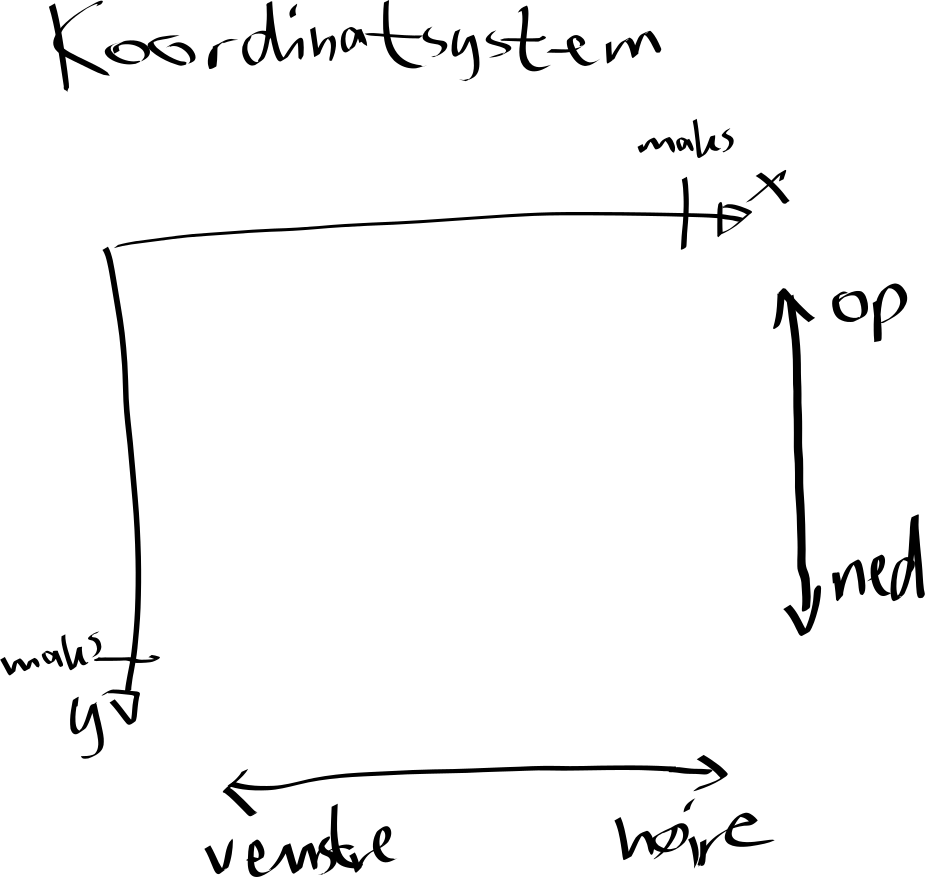
\includegraphics[width=\textwidth]{../brugere/kjaergaard/skaermkoordinater}
  \caption{Skærmkoordinater. Der arbejdes med skærmkoordinater i
    plotteren.}
  \label{fig:skaermkoord}
\end{figure}

\section{Timing \& Buffer}

I afsnittet om mekanik lå fokus meget på nøjagtigheden af vores
produkt. Vi vil her diskutere, hvordan vi vil opnå denne nøjagtighed.

Vi har diskuteret to løsninger. Den ene forgår ud af en såkaldt tråd,
hvor vi udfører og holder pause, udfører og holder pause. Dette giver
dog anledning til en forsinkelse. Dette kan ses på figur\fixme{indsæt
  figur af trådløsning}.  Da vi ikke kan bestemme forsinkelsen i
praksis, så er denne løsning ikke optimalt til vores projekt.

Vi kom herefter frem til en løsning, hvor vi benytter os af en buffer,
som man kan læse mere om under afsnittet Software under
Implementering. Her udføres instruktionerne, som er samlet i bufferen
sammen med et tidspunkt, når dette tidspunkt er overskredet. Der skal
altså jævnt udføres et tjek, som den såkaldte deadline er
overskredet. Imellem disse tjek kan bufferen få data.

Der er dog problemer, som vi skal tage højde for, når vi bruger en
buffer. F.eks. må hastigheden af outputtet ikke overskride
hastigeheden hvormed bufferen får data fra HPGL. Sagt mere simpel, så
må bufferen aldrig tømmes helt. Hvis dette sker, så har bufferen ikke
nok information eller jobs til motorstyringen, hvilket medfører en
overskrides af vores deadline, svarende til det tidspunkt vi skal have
udført vores funktion. Afstanden imellem to tjek skal skal således
være stor nok, så bufferen har tid til at modtage data. Dataen kommer
som sagt fra HPGL, som har behandlet information fra SD-kortet. Dette
ses illustreret i figur\fixme{Illustration som viser overførsel af
  data fra SD-kort osv.}.

Vi skal også tage højde for, at bufferen ikke nødvendigvis bliver
fyldt før hvert tjek. Dette giver anledning til et interrupt, hvor
opfyldningen af bufferen stoppes og tjekket udføres. Efter tjekket
genoptages opfyldningen af bufferen. Brugen af en buffer har den
fordel, at hastigheden af output er nogenlunde konstant. Diagrammet
over brugen af en buffer kan ses i figur\fixme{indsæt figur over
  bufferforløb}.



\section{Valg af programmeringssprog}

Softwaren skrives i C og C++.

C bruges i moduler, hvor sproget uden videre er tilstrækkeligt. Dette
vil typisk være lavniveaumoduler, og her er C fordelagtigt, fordi det
giver større kontrol.

C++ bruges i moduler, hvor det er fordelagtigt at bruge C++-speficikke
elementer (f.eks. generisk programmering\fixme{note om
  dette?}). Moduler, der afhænger af moduler skrevet i C++, vil typisk
også være skrevet i C++.

Alle C-moduler er kompatible med C++, og alle C++-moduler er så vidt
muligt kompatible med C. Uønskede sideeffekter af C++ forsøges undgået
(\fixme{eksempler her!}). C++ bruges ikke objektorienteret.



%%% Local Variables: 
%%% mode: latex
%%% TeX-master: "../master"
%%% End:\section{Koordinatsystem}